
\newcommand{\insimg}[1] {
  \begin{subfigure}[b]{0.2\textwidth}
    \centering
    \includegraphics[keepaspectratio=true, width=\textwidth]{images/#1}
  \end{subfigure}
}

\chapter{性能测试}
\label{chap:benchmark}

为了测试本系统的可用性,需要测试检索算法的鲁棒性、效率以及正确率。

\section{测试指标}
\label{sec:benchmark-index}

\begin{itemize}
\item \textbf{鲁棒性}:本系统利用DCT抽取出图像的特征向量,采用向量间的距离作为图
  片的相似程度的度量,距离越大,图片相似程度越低,同理,距离越小(大
  于0),图片的相似程度就越高。对鲁棒性的测试应着眼于在不同情况下,加噪
  图与原图的距离的变化情况,距离越小,抗噪声性能越好。

\item \textbf{效率}:本系统接受一个待检索图后,在特征数据库中检索所有的特征向量
  后返回前10相似的图片。对效率的测试应着眼于系统检索出结果的时间,以及
  客户端接收到全部结果图片的时间,检索时间越小,服务端检索性能越好,接
  受时间越小,客户端性能越好。

\item \textbf{检索正确率}:检索结果与原图在内容上的相关性,相关性越高,正确率越
  高。检索结果图与原图是否相关由人工判断。
\end{itemize}
\section{测试方案}
\label{sec:benchmark-scheme}

\begin{itemize}
\item 为了测试检索算法的鲁棒性,拟选择一些样本图片,并对这些样本做一些典型的
变化:
\begin{itemize}
\item 加入椒盐噪声
\item 改变质量因子$Q$
\end{itemize}
然后统计加噪图与原图的距离。

\item 为了测试检索算法的效率,拟在同一台主机上同时开启本系统的服务端和客户端,
即在忽略网络状况的情况下测试系统的检索速度并统计时间。

\item 为了测试检索算法的检索正确率,拟选择所有样本图片的标准图,并用这
  些标准图做检索,随后统计出结果集与原标准图的相关性。
\end{itemize}

\section{测试环境}
\label{sec:benchmark-env}

\begin{itemize}
  \item \textbf{硬件环境}
  \begin{itemize}
    \item Intel Core i5-2410M CPU @ 2.30GHz
    \item 4.00GB RAM(3.82GB可用)
  \end{itemize}
  \item \textbf{软件环境}
  \begin{itemize}
    \item Windows 8 专业版 x64(含Media Center) 
    \item Python 2.7.3 x86
    \item numpy 1.7.1
    \item opencv-python-2.4.5
  \end{itemize}
\end{itemize}

\section{测试数据}
\label{sec:benchmark-data}

测试图像集为40张灰度正脸无表情人脸图(即标准图)与他们的其他表情或姿势
人脸图\cite{dataset},大小为$640 \times 480$,单位为像素。标准图集如下图

\begin{figure}[H]
  \centering
  \insimg{gs0.jpg}
  \insimg{gs1.jpg}
  \insimg{gs2.jpg}
  \insimg{gs3.jpg}
  \vspace{0.1cm}

  \insimg{gs4.jpg}
  \insimg{gs5.jpg}
  \insimg{gs6.jpg}
  \insimg{gs7.jpg}
  \vspace{0.1cm}

\end{figure}
\begin{figure}[H]
  \centering

  \insimg{gs8.jpg}
  \insimg{gs9.jpg}
  \insimg{gs10.jpg}
  \insimg{gs11.jpg}
  \vspace{0.1cm}

  \insimg{gs12.jpg}
  \insimg{gs13.jpg}
  \insimg{gs14.jpg}
  \insimg{gs15.jpg}
  \vspace{0.1cm}

  \insimg{gs16.jpg}
  \insimg{gs17.jpg}
  \insimg{gs18.jpg}
  \insimg{gs19.jpg}
  \vspace{0.1cm}

  \insimg{gs20.jpg}
  \insimg{gs21.jpg}
  \insimg{gs22.jpg}
  \insimg{gs23.jpg}
  \vspace{0.1cm}

  \insimg{gs24.jpg}
  \insimg{gs25.jpg}
  \insimg{gs26.jpg}
  \insimg{gs27.jpg}
  \vspace{0.1cm}

  \insimg{gs28.jpg}
  \insimg{gs29.jpg}
  \insimg{gs30.jpg}
  \insimg{gs31.jpg}
  \vspace{0.1cm}

  \insimg{gs32.jpg}
  \insimg{gs33.jpg}
  \insimg{gs34.jpg}
  \insimg{gs35.jpg}
  \vspace{0.1cm}

  \insimg{gs36.jpg}
  \insimg{gs37.jpg}
  \insimg{gs38.jpg}
  \insimg{gs39.jpg}
  \vspace{0.1cm}
\end{figure}

以1号人物为例,以下列举类型编号:
\begin{itemize}
\item \textbf{类型1}:正脸全图,无表情,漫射光,即标准图
  \begin{figure}[H]
    \centering
    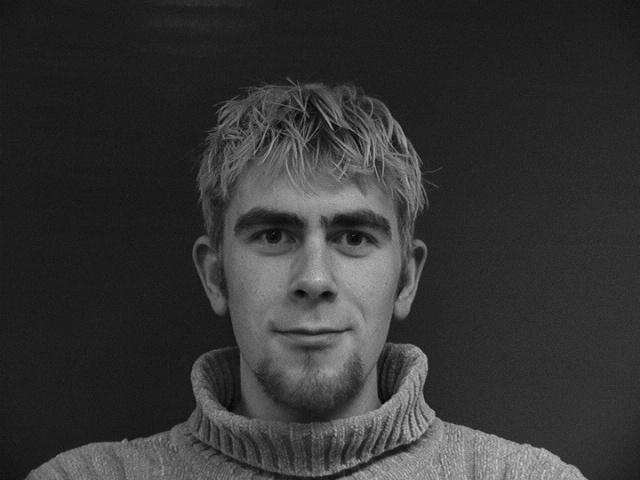
\includegraphics[keepaspectratio=true,
    scale=0.33]{images/gs0/gs0.jpg}
  \end{figure}
\item \textbf{类型2}:正脸全图,“高兴”的表情,漫射光
  \begin{figure}[H]
    \centering
    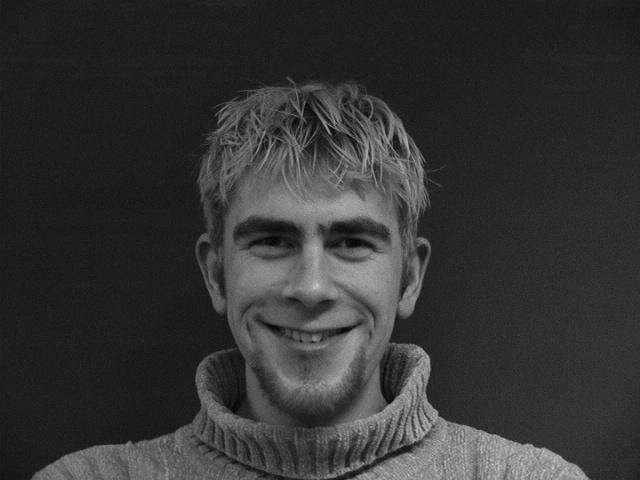
\includegraphics[keepaspectratio=true,
    scale=0.33]{images/gs0/gs1.jpg}
  \end{figure}
\item \textbf{类型3}:30度人物右转,无表情,漫射光
  \begin{figure}[H]
    \centering
    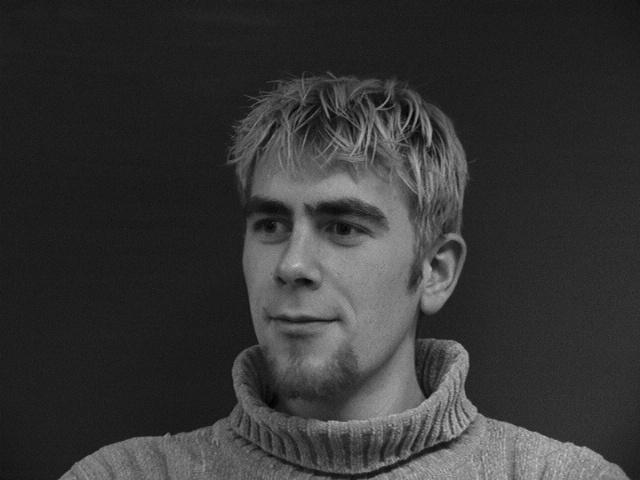
\includegraphics[keepaspectratio=true,
    scale=0.33]{images/gs0/gs2.jpg}
  \end{figure}
\item \textbf{类型4}:30度人物左转,无表情,漫射光
  \begin{figure}[H]
    \centering
    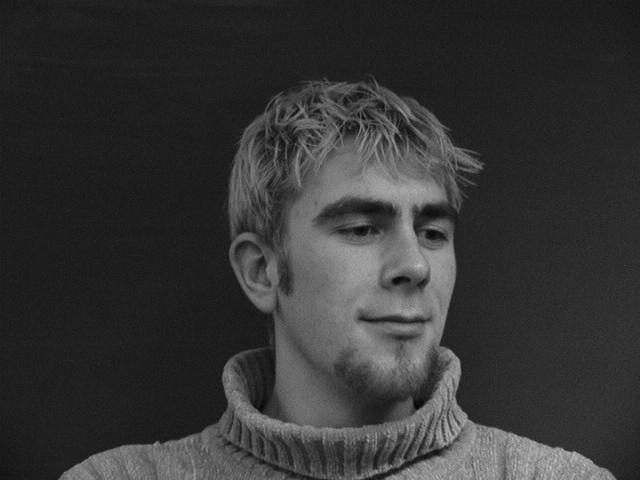
\includegraphics[keepaspectratio=true,
    scale=0.33]{images/gs0/gs3.jpg}
  \end{figure}
\item \textbf{类型5}:正脸全图,无表情,人物左侧增加投光灯
  \begin{figure}[H]
    \centering
    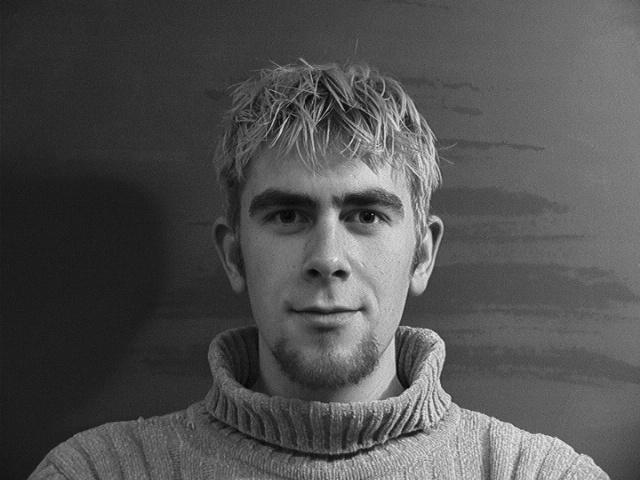
\includegraphics[keepaspectratio=true,
    scale=0.33]{images/gs0/gs4.jpg}
  \end{figure}
\item \textbf{类型6}:正脸全图,任意表情,漫射光
  \begin{figure}[H]
    \centering
    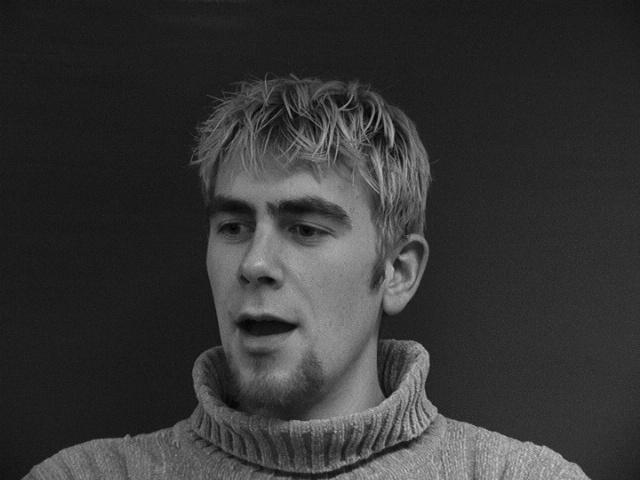
\includegraphics[keepaspectratio=true,
    scale=0.33]{images/gs0/gs5.jpg}
  \end{figure}
\end{itemize}

\section{测试结果及分析}
\label{sec:result-and-analysis}

\subsection{椒盐噪声}
\label{sec:speckle-data}

典型的加入椒盐噪声的图如下
\begin{figure}[H]
  \centering
  \begin{subfigure}[b]{0.4\textwidth}
    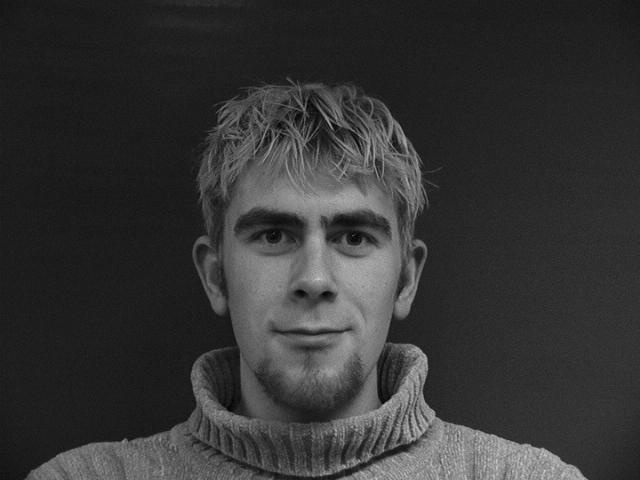
\includegraphics[keepaspectratio=true,
    width=\textwidth]{images/gs0.jpg}
    \caption{原图}
  \end{subfigure}
  \begin{subfigure}[b]{0.4\textwidth}
    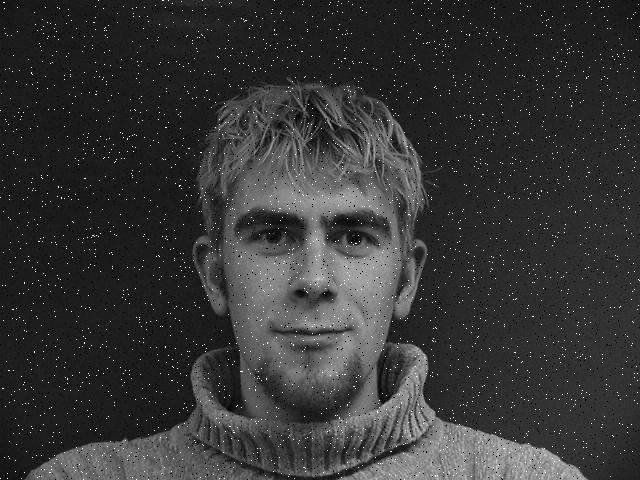
\includegraphics[keepaspectratio=true,
    width=\textwidth]{images/gs0_0.02_speckle.jpg}
    \caption{加噪图}
  \end{subfigure}
  \caption{噪声参数为0.02时的椒盐噪声对gs0.jpg的影响}
\label{fig:speckle-ex-img}
\end{figure}

对上示原图加入噪声密度在$[0, 0.1]$内、步长为0.01的椒盐噪声后,分别统计
与原图的距离,可作如下的散点图
\begin{figure}[H]
  \centering
  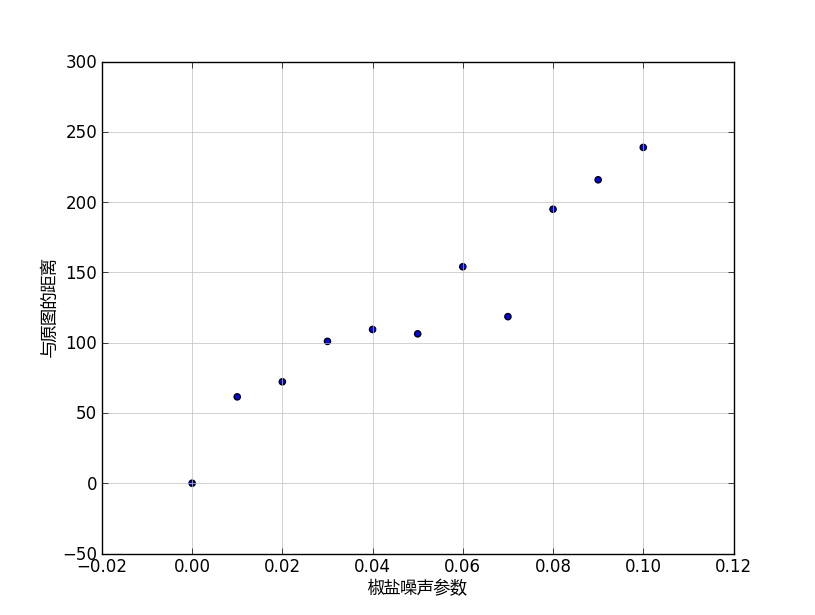
\includegraphics[keepaspectratio=true,
  scale=0.6]{images/speckle_gs0.png}
  \caption{对gs0.jpg的椒盐噪声统计}
  \label{fig:speckle-gs0-scatter-plot}
\end{figure}

为不失一般性,选取标准图集做同样处理,统计出散点图,如图
\begin{figure}[H]
  \centering
  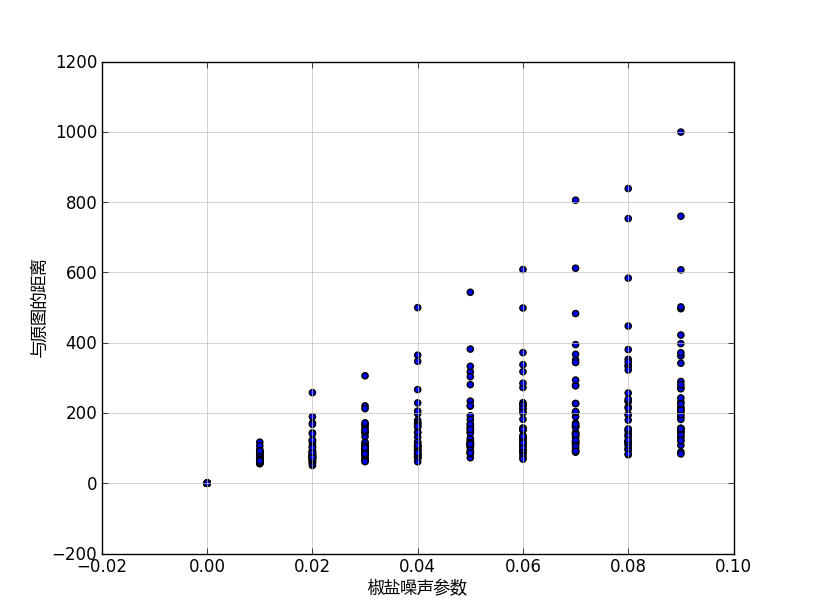
\includegraphics[keepaspectratio=true,
  scale=0.6]{images/speckle_all.png}
  \caption{对所有图片的椒盐噪声统计}
  \label{fig:speckle-all-scatter-plot}
\end{figure}

从图中可以看出来,本算法可以抵抗噪声密度小于$0.1$的椒盐噪声,在此噪声
密度下,加噪图与原图距离普遍小于$500$,当噪声密度大于$0.1$后,加噪图
与原图距离增大到了无法接受的地步。

\subsection{质量因子}
\label{sec:quality-data}

原图与质量因子$Q = 10$时的图如下
\begin{figure}[H]
  \centering
  \begin{subfigure}[b]{0.4\textwidth}
    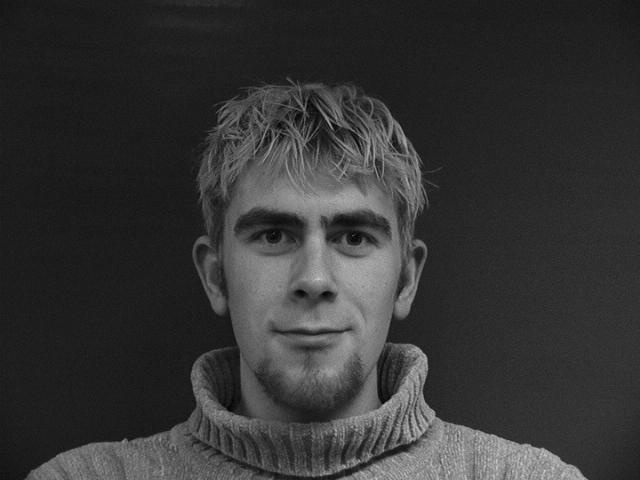
\includegraphics[keepaspectratio=true,
    width=\textwidth]{images/gs0.jpg}
    \caption{原图}
  \end{subfigure}
  \begin{subfigure}[b]{0.4\textwidth}
    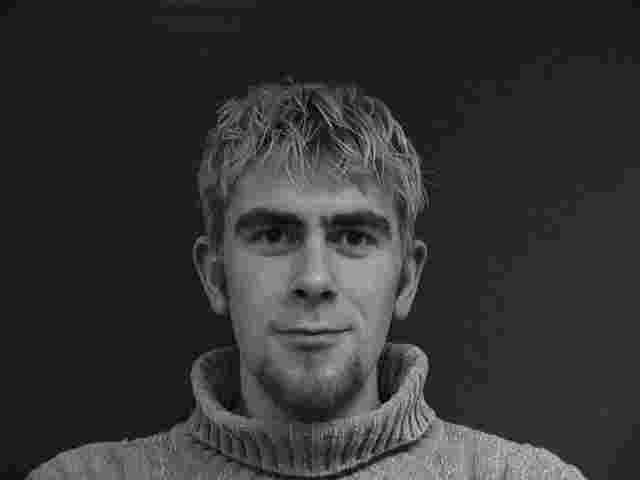
\includegraphics[keepaspectratio=true,
    width=\textwidth]{images/gs0_0.10_quality.jpg}
    \caption{压缩图}
  \end{subfigure}
  \caption{质量因子为10时的压缩操作对gs0.jpg的影响}
\label{fig:quality-ex-img}
\end{figure}

调整上示原图的质量因子$Q \in [0, 1]$、步长为$0.1$(在$[0.9, 1]$之间步长
为$0.01$)后,分别统计与原图的距离,可作如下的散点图
\begin{figure}[H]
  \centering
  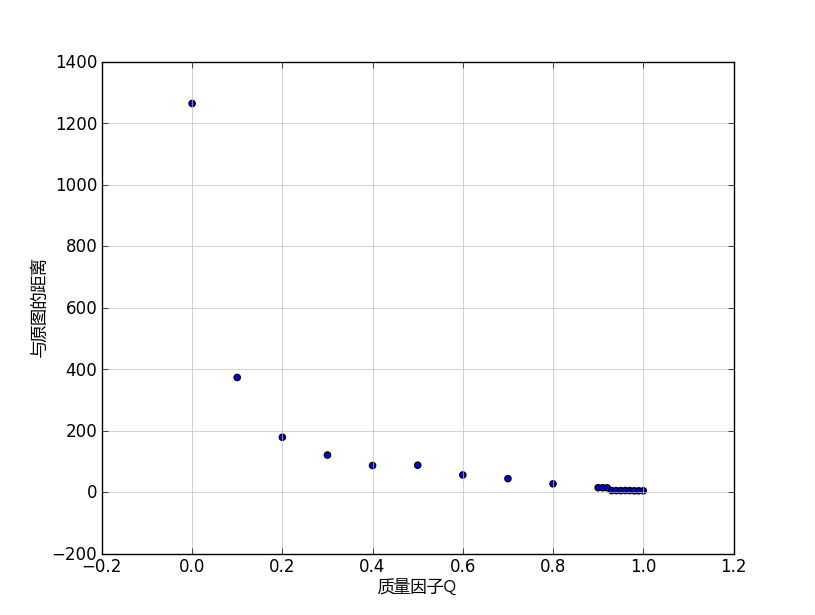
\includegraphics[keepaspectratio=true,
  scale=0.6]{images/quality_gs0.png}
  \caption{对gs0.jpg的压缩操作统计}
  \label{fig:quality-gs0-scatter-plot}
\end{figure}

\begin{figure}[H]
  \centering
  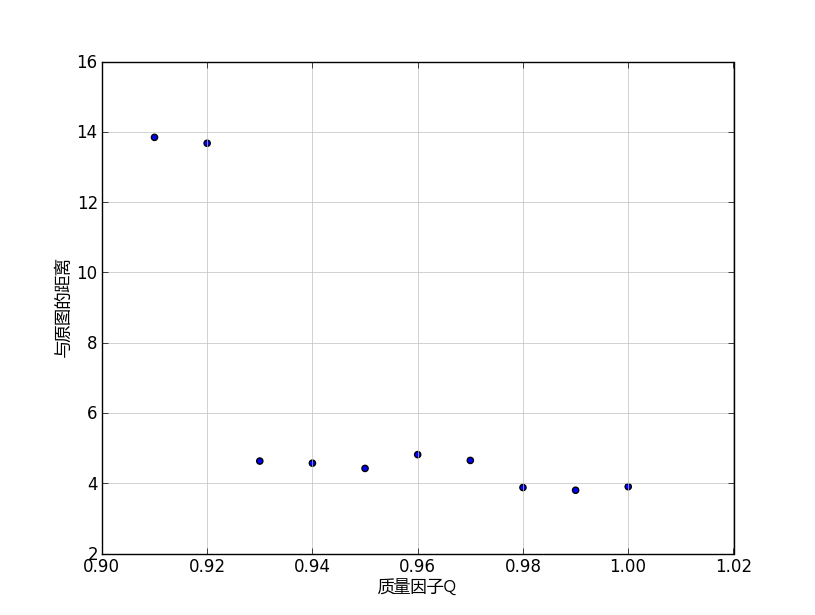
\includegraphics[keepaspectratio=true,
  scale=0.6]{images/quality_gs0_0.9_1.png}
  \caption{对gs0.jpg的压缩操作统计($[0.9, 1]$区间)}
  \label{fig:quality-gs0-sub-scatter-plot}
\end{figure}

为不失一般性,选取标准图集做同样处理,统计出散点图,如图
\begin{figure}[H]
  \centering
  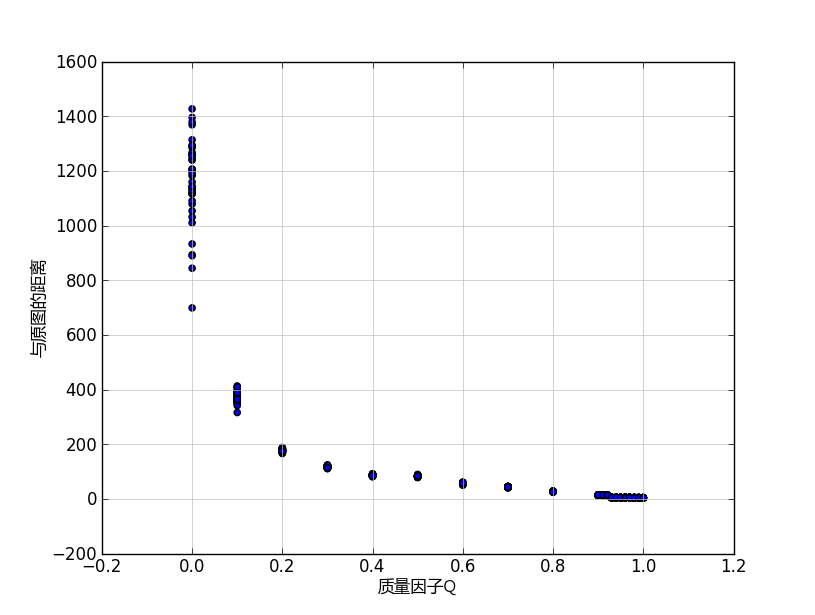
\includegraphics[keepaspectratio=true,
  scale=0.6]{images/quality_all.png}
  \caption{对所有图片的压缩操作统计}
  \label{fig:quality-all-scatter-plot}
\end{figure}

\begin{figure}[H]
  \centering
  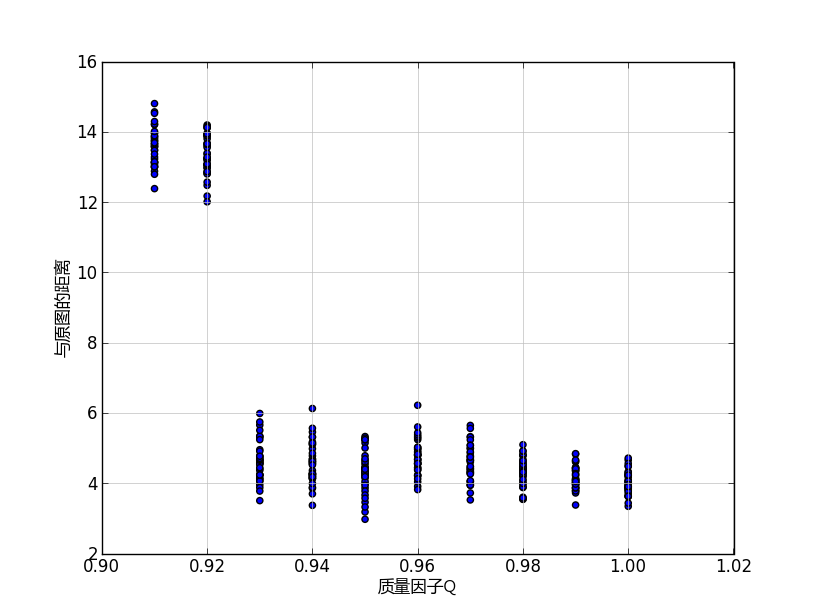
\includegraphics[keepaspectratio=true,
  scale=0.6]{images/quality_all_0.9_1.png}
  \caption{对所有图片的压缩操作统计($[0.9, 1]$区间)}
  \label{fig:quality-gs0-sub-scatter-plot}
\end{figure}

从图中可以看出来,本算法有较好的抗压缩性能,即使图片质量被调整为$10\%$,
与原图的距离仍然小于$500$。

\subsection{系统检索效率}
\label{sec:sys-retrieval-effi}

使用gs0.jpg做10次检索,分别记录:
\begin{itemize}
  \item \textbf{检索耗时$t_r$}:服务器比对所有特征向量,获得结果集所花时间;
  \item \textbf{检索结束耗时$t_a$}:客户端从点击\texttt{Retrieve}按钮开始到所有结
    果图像获取结束所花时间。
\end{itemize}

测试结果如下表


\begin{table}[H]
  \setlength{\tabcolsep}{25pt}
  \centering
  \begin{tabular}{ l c c }
    \hline
    序号 & $t_r$ & $t_a$ \\ \hline \hline
    1 & $0.08562$ & $3.44197$ \\
    2 & $0.08107$ & $3.50858$ \\
    3 & $0.08263$ & $3.42089$ \\
    4 & $0.08283$ & $3.46747$ \\
    5 & $0.08285$ & $3.50209$ \\
    6 & $0.11238$ & $3.50387$ \\
    7 & $0.08241$ & $3.43419$ \\
    8 & $0.08106$ & $3.50417$ \\
    9 & $0.08139$ & $3.44271$ \\
    10 & $0.08165$ & $3.46871$ \\
    均值 & $0.08539$ & $3.46947$ \\
    \hline
  \end{tabular}
  \caption{系统效率测试结果}
  \label{tab:sys-retrieval-effi}
\end{table}



该表显示出本系统的检索耗时$t_r$较小,即服务端检索性能较好,但检索结束
耗时$t_a$高出$t_r$很多,原因可能是base64加解码与图像加解密比较耗时。

\subsection{系统检索正确率}
\label{sec:sys-retrieval-correct-rate}

取标准图集中的每张图片做检索,分别统计出返回的结果集(距离
前10小\footnote{由于原图与原图自己距离为0,所以实际有效结果为前9小,检
  索出的类型也只有类型2到类型6})中

\begin{itemize}
  \item 与原图为同一人的个数$n_{count}$;
  \item 结果集中与原图为同一人的结果的最小序号$n_{label}$;
  \item 检索出的图片类型编号,其中编号按与原图的距离大小升序排序。
\end{itemize}


测试结果如下表


\begin{center}
    \setlength{\tabcolsep}{25pt}
  \begin{longtable}{ l c c c r }

    \hline \textbf{序号} & \textbf{性别} & \textbf{$n_{count}$} &
    \textbf{$n_{label}$} & \textbf{类型} \\
    \hline \hline
    \endfirsthead
    \multicolumn{5}{r}{\textit{接上页}} \\
    \hline
    \textbf{序号} & \textbf{性别} & \textbf{$n_{count}$} & \textbf{$n_{label}$} & \textbf{类型} \\
    \hline \hline
    \endhead
    \hline
    \endfoot
    \endlastfoot

    1 & M & 2 & 4 & 6, 2\\
    2 & M & 2 & 2 & 2, 4 \\
    3 & M & 3 & 1 & 4, 3, 2 \\
    4 & M & 4 & 1 & 3, 4, 6, 5 \\
    5 & M & 4 & 1 & 3, 2, 4, 6 \\
    6 & M & 4 & 1 & 4, 6, 3, 2 \\
    7 & M & 5 & 1 & 3, 4, 6, 2, 5 \\
    8 & F & 2 & 2 & 3, 2 \\
    9 & M & 3 & 3 & 4, 2, 3 \\
    10 & M & 1 & 4 & 2 \\
    11 & M & 4 & 1 & 4, 2, 3, 6 \\
    12 & F & 5 & 1 & 3, 4, 5, 2, 6 \\
    13 & M & 0 & n/a & n/a \\
    14 & F & 0 & n/a & n/a \\
    15 & F & 0 & n/a & n/a \\
    16 & M & 0 & n/a & n/a \\
    17 & M & 2 & 4 & 3, 4 \\
    18 & M & 5 & 1 & 3, 4, 6, 5, 2 \\
    19 & M & 1 & 9 & 2 \\
    20 & M & 3 & 3 & 3, 4, 2 \\
    21 & M & 3 & 1 & 2, 3, 6 \\
    22 & F & 2 & 1 & 4, 2 \\
    23 & M & 0 & n/a & n/a \\
    24 & M & 1 & 9 & 4 \\
    25 & M & 2 & 6 & 3, 2 \\
    26 & M & 0 & n/a & n/a \\
    27 & M & 3 & 2 & 2, 6, 3 \\
    28 & M & 3 & 1 & 6, 2, 3 \\
    29 & M & 1 & 9 & 3 \\
    30 & F & 0 & n/a & n/a \\
    31 & M & 2 & 1 & 2, 6 \\
    32 & F & 1 & 1 & 4 \\
    33 & M & 1 & 1 & 2 \\
    34 & M & 2 & 1 & 4, 3 \\
    35 & F & 2 & 4 & 4, 2 \\
    36 & M & 0 & n/a & n/a \\
    37 & M & 3 & 2 & 2, 3, 4 \\
    38 & M & 1 & 5 & 4 \\
    39 & M & 3 & 1 & 3, 4, 2 \\
    40 & M & 0 & n/a & n/a \\
    \hline
  \caption{系统正确率测试结果} \\
  \end{longtable}

  \label{tab:sys-retrieval-correct-rate}
\end{center}



分析上表数据,可得:
\begin{itemize}
  \item 检索成功次数31,失败次数(无与原图相关的结果)9,成功率$77.5\%$;
  \item 若检索成功,平均相关结果数$2.58$个;
  \item 平均最小编号$2.48$;
\end{itemize}

另外,各图片类型统计如下表


\begin{table}[H]
  \setlength{\tabcolsep}{25pt}
  \centering
  \begin{tabular}{ l c r }
    \hline
    \textbf{类型} & \textbf{次数} & \textbf{比例} \\ \hline \hline
    2 & 21 & $28.77\%$ \\
    3 & 19 & $26.03\%$ \\
    4 & 18 & $24.66\%$ \\
    5 & 4 & $5.48\%$ \\
    6 & 11 & $15.07\%$ \\
    总计 & 73 & $100.01\%$ \\
    \hline
  \end{tabular}
  \caption{图片类型统计}
  \label{tab:sys-retrieved-img-type}
\end{table}



可以看出背景光源对本算法影响较大,人物表情与脸部所朝方向影响稍小。

